Mini-Hubo\cite{threeTier} is a miniture version of the Hubo platform discribe in Section~\ref{sec:hubo}.
It is used as the Test and Evaluation (T\&E) stage of the three tier infrastructure discribed in Section~\ref{sec:threeTier}.
Mini-Hubo is kinematically scaled to the Hubo platform.
The atrobutes of the Mini-Hubo system are in Table~\ref{table:huboMiniSensors}.
The robot is shown in Fig.~\ref{fig:mini-hubo}


\begin{table}
\centering
\caption{Mini-Hubo Platform Specifications}
\begin{tabular}{| l || l |}
\hline
Height      		& $46~cm$			\\
\hline
Weight			& $2.9~kg$			\\
\hline
DOF			& 22				\\
\hline
Joint Control Type	& PID Position			\\
\hline
Computer		& $1.6~Ghz$ Atom		\\
			& $2~Gb$ DDR2 RAM		\\
\hline
Operating System	& Debian Linux			\\
\hline
Battery			& $14.8V$ $3.2~Ah$ $30C$ LiPo	\\
\hline
Sensors			& 2x 3 Axis Force Torque	\\
\hline
Vision			& Monocular			\\
			& RGBD				\\
\hline
\end{tabular}
\label{table:huboMiniSensors}
\end{table}





\begin{figure}[thpb]
  \centering
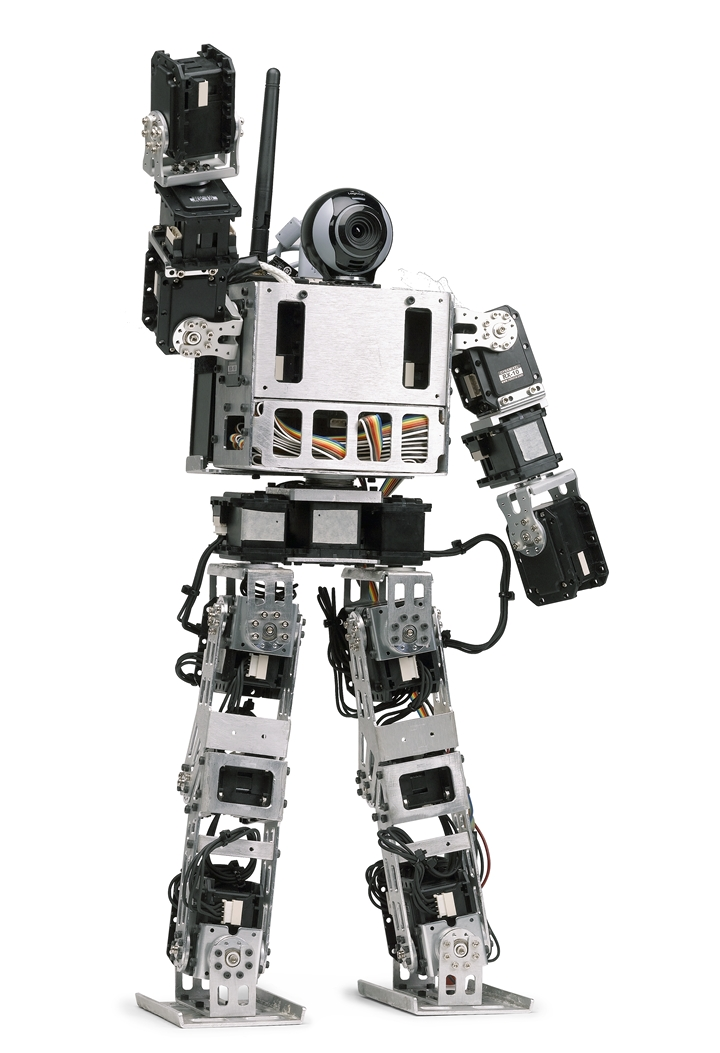
\includegraphics[width=0.37\columnwidth]{./pix/mini-hubo.jpg}
  \caption{Mini-Hubo platform: 22 DOF, 46 $cm$ tall miniture-size humanoid robot weighing 2.9 $kg$.}
  \label{fig:mini-hubo}
\end{figure}
